\section{Experiments} \label{sec:experiments}
%We conduct extensive experiments to validate the effectiveness of our proposed GeoPredict. Our evaluation is designed to answer several key research questions:

%\begin{enumerate}
    %\item How does GeoPredict perform against our $\pi_0$~\cite{black2410pi0} baseline and other state-of-the-art VLA models on complex long-horizon manipulation benchmarks? We present the corresponding quantitative results on RoboCasa~\cite{nasiriany2024robocasa} and LIBERO~\cite{liu2023libero} benchmarks in Sec.~\ref{sec:main_results}.

    %\item What is the specific contribution of each novel component introduced in our methodology, particularly the trajectory-level kinematic prediction and the predictive 3D Gaussian Splatting world model? We analyze the individual impact of these components through a detailed ablation study in Sec.~\ref{sec:ablations}.

    %\item Does the \textit{Track-based Gaussian Refinement} step measurably improve performance and training efficiency? We investigate this question through quantitative experiments in Sec.~\ref{sec:ablations}, demonstrating its ability to reduce training time while boosting success rates, and provide a visual analysis of the refinement quality in Sec.~\ref{sec:qualitative}.

    %\item How well do the benefits observed in simulation transfer to real-world robotic tasks, especially those demanding precise geometric and spatial reasoning? We report the results on our real-world evaluation suite in Sec.~\ref{sec:real_world}.
%\end{enumerate}

%\noindent We first introduce our experimental setup in Sec.~\ref{sec:exp_setup}.


We first introduce our experimental setup (Sec.~\ref{sec:exp_setup}), followed by a benchmarking against state-of-the-art baselines (Sec.~\ref{sec:main_results}). We then dissect the contribution of our proposed modules through detailed ablation studies (Sec.~\ref{sec:ablations}) and qualitative analysis (Sec.~\ref{sec:qualitative}). Finally, we assess the model's performance in real-world scenarios (Sec.~\ref{sec:real_world}).

\subsection{Experimental Setup} \label{sec:exp_setup}

\noindent \textbf{Simulation Benchmarks.}
We evaluate our method on two widely recognized robotic manipulation benchmarks.
\begin{itemize}[nolistsep, topsep=0pt, itemsep=1pt, parsep=0pt]
    \item \textbf{RoboCasa}~\cite{nasiriany2024robocasa}: This benchmark features 24 complex long-horizon everyday tasks in kitchen environments. We adopt the challenging \texttt{Human-50} few-shot setting, where policies are trained using only 50 human demonstrations per task. To rigorously assess generalization capabilities, we follow the standard protocol by evaluating our model over 50 trials per task across five distinct scenes. This evaluation is conducted exclusively on \textit{unseen object instances}, and includes scenes with \textit{unseen styles} that were never encountered during training.
    
    \item \textbf{LIBERO}~\cite{liu2023libero}: This benchmark is designed to evaluate knowledge transfer and policy generalization across four distinct task suites: LIBERO-Spatial, LIBERO-Object, LIBERO-Goal, and LIBERO-Long. We follow the standard protocol for LIBERO, training policies on 50 human-teleoperated demonstrations for each task and evaluating over 50 trials per task (500 trials per suite).
\end{itemize}


\noindent \textbf{Real-world Evaluation Suite.}
To evaluate GeoPredict's efficacy on real-world tasks requiring precise 3D reasoning, we use an evaluation suite (Figure~\ref{fig:real}). This suite includes three task categories, using 50 expert trajectories per category for training. Each policy is evaluated for 20 trials per category, where success is defined as successfully grasping the target object and placing it in the correct position.

\begin{itemize}[nolistsep, topsep=0pt, itemsep=1pt, parsep=0pt]
    \item \textbf{Spatial Generalization:} The robot is instructed to place the green cube into a plate. We evaluate the policy with the plate located at positions \textit{unseen} during training, testing its ability to generalize to novel target locations.

    \item \textbf{Geometry Generalization:} During the 20 evaluation trials, the model must grasp four distinct object types: a small cube, a medium cube, a large cube, and a rectangular prism. Critically, the test set includes cubes with dimensions \textit{not seen} during training. Furthermore, the rectangular prism is tested in its three unique stable orientations, requiring the policy to adapt its grasp approach based on the perceived object geometry.

    \item \textbf{Visual Robustness:} This task evaluates the policy's resilience to visual distractors. The robot must place the yellow cube into the plate while novel and task-irrelevant objects are introduced into the background of the scene, which were absent during training.
\end{itemize}

\begin{figure}[t]
  \centering
  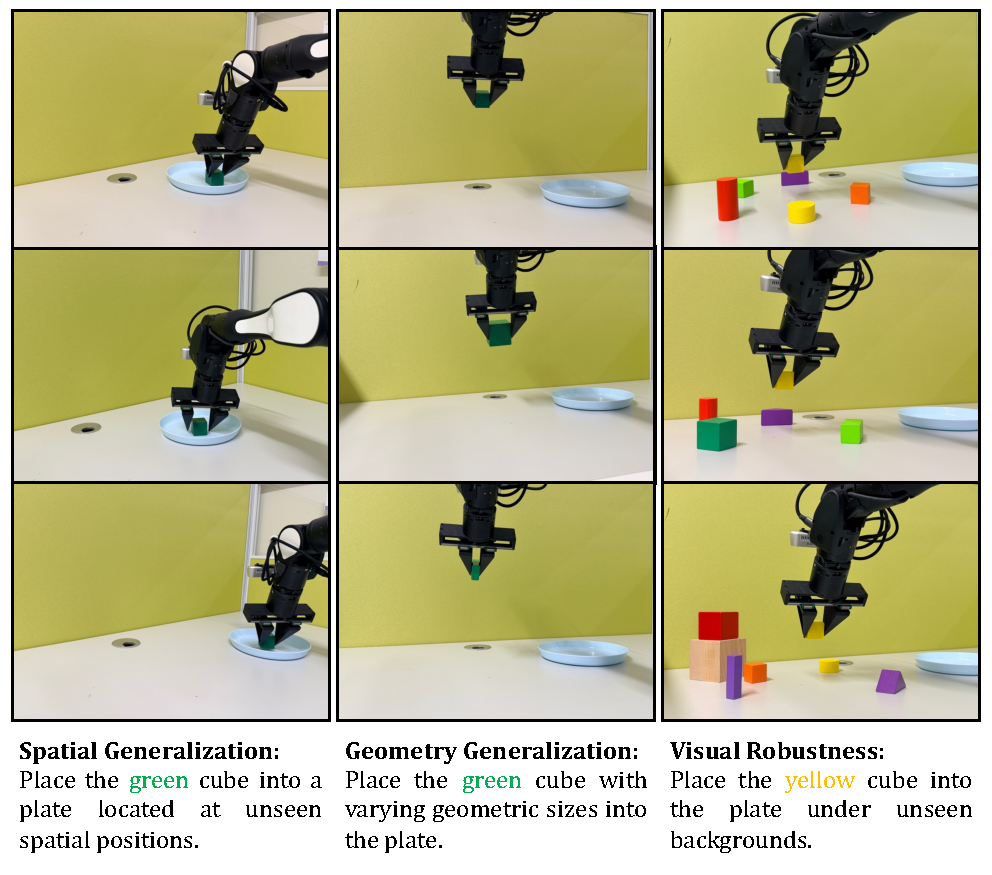
\includegraphics[width=0.47\textwidth]{fig/real.pdf}
  \vspace{-5pt}
  \caption{\textbf{Real-world Evaluation Suite.} These settings aim to evaluate the model's spatial generalization, geometry generalization and robustness to distractors. Each column represents different trials of the same task.}
  \label{fig:real}
  \vspace{-10pt}
\end{figure}

% 多次随机种子得到结果，详细的标准差结果见附录
\begin{table*}[htbp]
\caption{\textbf{RoboCasa Simulation Benchmark Results.} Task success rates (\%) across 24 sub-tasks and the Average Success Rate (\%). $^{\bm{\ast}}$Denotes our fine-tuned experimental results. \textbf{Bold} indicates the best performing model. See Appendix for detailed sub-task definitions.}
\vspace{-5pt}
\centering
\small
\begin{tabular}{l|cccccccccccc} 
\toprule
\multirow{2}{*}{\textbf{Method}} & \textbf{PnP} & \textbf{PnP} & \textbf{PnP} & \textbf{PnP} & \textbf{PnP} & \textbf{PnP} & \textbf{PnP} & \textbf{PnP} & \textbf{CM} & \textbf{CM} & \textbf{CB} & \multirow{2}{*}{\textbf{TSS}} \\
 & \textbf{CTC1} & \textbf{CTC2} & \textbf{CTS1} & \textbf{STC1} & \textbf{CTS2} & \textbf{STC2} & \textbf{CTM} & \textbf{MTC} & \textbf{SU} & S\textbf{V} & \textbf{PS} & \\ 
\midrule

BC-Transformer~\cite{nasiriany2024robocasa}& 6.0 & 2.0 & 2.0 & 8.0 & 2.0 & 6.0 & 2.0 & 2.0 & 0.0 & 22.0 & 48.0 & 54.0 \\

GWM~\cite{lu2025gwm} & 4.0 & \textbf{18.0} & 20.0 & 22.0 & 2.0 & 18.0 & 14.0 & \textbf{20.0} & 16.0 & 36.0 & \textbf{76.0} & \textbf{72.0} \\

$\pi_0^{\bm{\ast}}$ (Baseline)~\cite{black2410pi0} & 24.0 & 6.8 & 26.8 & 15.6 & 11.2 & 12.8 & 6.8 & 7.6 & 18.4 & 33.6 & 74.0 & 69.6 \\

\textbf{GeoPredict (Ours)} & \textbf{32.4} & 8.8 & \textbf{27.6} & \textbf{31.2} & \textbf{20.4} & \textbf{28.8} & \textbf{14.4} & 18.0 & \textbf{28.4} & \textbf{49.2} & 67.6 & 70.8 \\

\midrule
\textbf{Average Success Rate} & 
\textbf{OSD} &
\textbf{CSD} &
\textbf{ODD} &
\textbf{CDD} &
\textbf{OD} &
\textbf{CD} &
\textbf{TNSF} &
\textbf{TFSF} &
\textbf{TNS} &
\textbf{TFS} &
\textbf{TNM} &
\textbf{TFM} \\
\midrule

\multicolumn{1}{c|}{28.8} & 46.0 & 56.0 & 28.0 & 28.0 & 42.0 & 80.0 & 38.0 & 50.0 & 32.0 & 4.0 & 62.0 & 70.0\\

\multicolumn{1}{c|}{39.2} & \textbf{58.0} & 54.0 & 28.0 & 50.0 & 56.0 & 80.0 & 52.0 & 44.0 & 46.0 & \textbf{22.0} & 64.0 & 70.0\\

\multicolumn{1}{c|}{42.3} & 40.8 & \textbf{82.0} & 55.2 & 69.2 & 66.4 & 96.0 & 43.6 & 86.0 & 43.2 & 6.0 & 59.6 & 60.0\\

\multicolumn{1}{c|}{\textbf{52.4}} & 40.4 & 78.8 & \textbf{87.2} & \textbf{70.0} & \textbf{77.6} & \textbf{96.8} & \textbf{72.4} & \textbf{94.8} & \textbf{60.0} & 13.2 & \textbf{84.8} & \textbf{82.8}\\

\bottomrule
\end{tabular}
\label{tab:robocasa}
\vspace{-5pt}
\end{table*}




\begin{table*}[htbp]
\centering
\small
\caption{\textbf{LIBERO Simulation Benchmark Results.} Task success rates (\%) across 4 evaluation suites and the Average Success Rate (\%). $^{\bm{\ast}}$Denotes our reproduced experimental results. $^{\bm{\dagger}}$Denotes no available standard deviation data. \textbf{Bold} indicates the \textbf{best} performing model, and \underline{underline} indicates the \textbf{runner-up} model.}
\vspace{-5pt}
\begin{tabular}{l | c  c  c  c | c}
\toprule
\textbf{Method} & 
\multicolumn{1}{c}{\textbf{LIBERO-Spatial}} & 
\multicolumn{1}{c}{\textbf{LIBERO-Object}} & 
\multicolumn{1}{c}{\textbf{LIBERO-Goal}} & 
\multicolumn{1}{c|}{\textbf{LIBERO-Long}} & 
\multicolumn{1}{c}{\textbf{Average}} \\
\midrule
Diffusion Policy~\cite{chi2025diffusion} & 78.3 $\pm$ 1.1 & 92.5 $\pm$ 0.7 & 68.3 $\pm$ 1.2 & 50.5 $\pm$ 1.3 & 72.4 $\pm$ 0.7 \\
TraceVLA~\cite{zheng2024tracevla} & 84.6 $\pm$ 0.2 & 85.2 $\pm$ 0.4 & 75.1 $\pm$ 0.3 & 54.1 $\pm$ 1.0 & 74.8 $\pm$ 0.5 \\
Octo~\cite{team2024octo} & 78.9 $\pm$ 1.0 & 85.7 $\pm$ 0.9 & 84.6 $\pm$ 0.9 & 51.1 $\pm$ 1.3 & 75.1 $\pm$ 0.6 \\
OpenVLA~\cite{kim2025openvla} & 84.7 $\pm$ 0.9 & 88.4 $\pm$ 0.8 & 79.2 $\pm$ 1.0 & 53.7 $\pm$ 1.3 & 76.5 $\pm$ 0.6 \\
SpatialVLA~\cite{qu2025spatialvla} & 88.2 $\pm$ 0.5 & 89.9 $\pm$ 0.7 & 78.6 $\pm$ 0.6 & 55.5 $\pm$ 1.0 & 78.1 $\pm$ 0.7 \\
WorldVLA$^{\bm{\dagger}}$~\cite{cen2025worldvla} & 87.6 & 96.2 & 83.4 & 60.0 & 81.8 \\
4D-VLA~\cite{zhang20254d} & 88.9 $\pm$ 0.5 & 95.2 $\pm$ 0.3 & 90.9 $\pm$ 0.4 & 79.1 $\pm$ 1.2 & 88.6 $\pm$ 0.3 \\
DreamVLA$^{\bm{\dagger}}$~\cite{zhangdreamvla} & \underline{97.5} & 94.0 & 89.5 & 89.5 & 92.6 \\
$\pi_0^{\bm{\dagger}}$~\cite{black2410pi0} & 96.8 & \textbf{98.8} & \textbf{95.8} & 85.2 & 94.2\\
OpenVLA-OFT$^{\bm{\dagger}}$~\cite{kim2025fine} & 95.2 & 94.2 & 95.2 & \underline{93.2} & 94.5 \\
UniVLA$^{\bm{\dagger}}$~\cite{bu2025univla} & 96.5 & 96.8 & 95.6 & 92.0 & \underline{95.2} \\
\midrule
$\pi_0^{\bm{\ast}}$ (Baseline)~\cite{black2410pi0} & 96.6 $\pm$ 0.6 & 97.2 $\pm$ 0.8 & 94.2 $\pm$ 0.7 & 87.6 $\pm$ 1.1 & 93.9 $\pm$ 0.4\\
\textbf{GeoPredict (Ours)} & \textbf{98.0 $\pm$ 0.7} & \underline{98.2 $\pm$ 0.7} & \underline{95.7 $\pm$ 0.2} & \textbf{94.0 $\pm$ 1.0} & \textbf{96.5 $\pm$ 0.6} \\
\bottomrule
\end{tabular}
\label{tab:libero}
\vspace{-10pt}
\end{table*}

\noindent \textbf{Baselines.}
Our primary baseline is our VLA backbone, \textbf{$\pi_0$}~\cite{black2410pi0}, trained without our proposed predictive 3D modules. This comparison directly isolates the contribution of our geometry-aware predictive method. We also compare against a range of state-of-the-art VLA and world-modeling approaches, including BC-Transformer~\cite{nasiriany2024robocasa}, GWM~\cite{lu2025gwm}, OpenVLA~\cite{kim2025openvla}, SpatialVLA~\cite{qu2025spatialvla} and UniVLA~\cite{bu2025univla}.


\noindent \textbf{Implementation Details.}
A predictive horizon of $H=50$ is used for all tasks. Observations include two environment and one wrist camera views. Depth supervision is applied only to the two $224\times224$ environment cameras. For the trajectory-level prediction module (Sec.~\ref{sec:track_query}), we track $K=8$ keypoints (7 joints, 1 end-effector) for LIBERO~\cite{liu2023libero} and RoboCasa~\cite{nasiriany2024robocasa}, and $K=7$ (6 joints, 1 end-effector) for the real-world setup. For the predictive 3DGS geometry module (Sec.~\ref{sec:3dgs}), the workspace is $1.6\text{m} \times 1.6\text{m} \times 1.0\text{m}$ with $v=0.04$m voxels. Token and decoder feature dimensions are $C=2048$ and $C'=256$. We use $N_G=4$ initial primitives per voxel, and generate $N_G'=64$ additional primitives for voxels selected by the track-guided refinement mechanism. All loss weights in Eq.~\eqref{eq:total_loss} are 1.0. We train for 40,000 iterations using AdamW~\cite{loshchilovdecoupled} (LR 2.5e-5) on 8 NVIDIA H20 GPUs with a total batch size of 32. The primary metric is Task Success Rate (\%).










\subsection{Main Results} \label{sec:main_results}

\noindent \textbf{RoboCasa.}
Table~\ref{tab:robocasa} details the performance across the 24 RoboCasa sub-tasks. GeoPredict achieves an average success rate of \textbf{52.4\%}, significantly outperforming all baselines. Notably, it improves upon the $\pi_0$ baseline success rate of 42.3\% by a margin of \textbf{10.1\%}. This substantial gain underscores the benefit of conditioning the policy on predictive kinematic and geometric priors, especially in the \texttt{Human-50} few-shot setting where generalization from limited data is critical~\cite{nasiriany2024robocasa}. Moreover, GeoPredict demonstrates clear advantages over other future prediction methods such as GWM~\cite{lu2025gwm} at 39.2\% and 2D policies like BC-Transformer~\cite{nasiriany2024robocasa} at 28.8\%. Additional large-scale results on RoboCasa \texttt{Generated-300} are in the Appendix.




\noindent \textbf{LIBERO.}
In Table~\ref{tab:libero}, we show results on the four LIBERO suites~\cite{liu2023libero}. GeoPredict achieves an average success rate of \textbf{96.5\%}, surpassing the current SOTA method UniVLA~\cite{bu2025univla}. Furthermore, it significantly outperforms strong baselines such as OpenVLA~\cite{kim2025openvla} which attains 76.5\% by a margin of 20.0\%. Our model demonstrates consistently high performance across all four suites, including Spatial (98.0\%), Object (98.2\%), Goal (95.7\%), and the challenging Long (94.0\%). This indicates that our method's geometry-aware training is highly effective and generalizes robustly across diverse tasks and environments.


\subsection{Ablation Study} \label{sec:ablations}
\noindent \textbf{Component Ablation.}
Table~\ref{tab:ab_module} details our ablation, building the model from the ground up. Starting from the $\pi_0$ baseline (42.3\%), adding the history Track Encoder provides a kinematic prior, improving performance to 44.8\%. Adding the Future Track Query ($\mathcal{L}_{track}$) for explicit motion prediction further boosts the rate to 47.2\%.

The predictive 3D Gaussian Splatting geometry module yields the most substantial gains. Supervising with $\mathcal{L}_{depth}$ (using only initial $\mathbf{G}^{init}$) elevates performance to 49.4\%. Jointly training with $\mathcal{L}_{track}$ and $\mathcal{L}_{depth}$ but without the explicit \textit{track-guided refinement} yields 50.5\%. Critically, activating the full \textit{track-guided refinement} mechanism, which allocates geometric capacity along the predicted future tracks, achieves the peak 52.4\%. This final 1.9\% gain (50.5\% $\to$ 52.4\%) validates our hypothesis: using kinematic predictions to refine the 3DGS representation provides a superior geometric prior for the policy.

\noindent \textbf{Ablation on Depth Rendering.}
Table~\ref{tab:ab_depth} ablates our predictive 3DGS method. Rendering with color (49.2\%) offers no benefit over depth-only (49.4\%), confirming geometric information alone suffices. Increasing the global initial primitives from $N_G=4$ to $N_G=8$ (51.4\%) significantly increases training time (12.0 to 19.1 hours/epoch).

In contrast, our \textit{track-guided refinement} strategy ($N_G=4, N_G'=8$) is more efficient, achieving 51.1\% at only 15.5 hours/epoch. This highlights the efficiency of allocating geometric capacity to task-relevant interaction regions. Since these regions are a small fraction of the volume, we can increase $N_G'$ with negligible overhead. Setting $N_G'=64$ yields our peak 52.4\% success rate at a near-identical 15.7 hours. Therefore, we adopt $N_G=4$ and $N_G'=64$ as our final configuration.

\begin{table}[t]
\centering
\small
\caption{\textbf{Ablation Study on RoboCasa Simulation Benchmark.} Future Depth is rendered from initial global Gaussians ($\textbf{G}^{init}$), while Future Depth$^{\bm{\ast}}$ utilizes the refined total Gaussians ($\textbf{G}^{total}$). Results denote the Average Success Rate (\%) across all sub-tasks.}
\vspace{-5pt}
\begin{tabular}{l | c  c  c  c c c}
\toprule
History Track & \textcolor{red}{\ding{56}} & \textcolor{blue}{\ding{52}} & \textcolor{blue}{\ding{52}} & \textcolor{red}{\ding{56}} & \textcolor{blue}{\ding{52}} & \textcolor{blue}{\ding{52}}\\
Future Track & \textcolor{red}{\ding{56}} & \textcolor{red}{\ding{56}} & \textcolor{blue}{\ding{52}} & \textcolor{red}{\ding{56}} & \textcolor{blue}{\ding{52}} & \textcolor{blue}{\ding{52}}\\
Future Depth & \textcolor{red}{\ding{56}} & \textcolor{red}{\ding{56}} & \textcolor{red}{\ding{56}} & \textcolor{blue}{\ding{52}} & \textcolor{blue}{\ding{52}} & \textcolor{red}{\ding{56}}\\
Future Depth$^{\bm{\ast}}$ & \textcolor{red}{\ding{56}} & \textcolor{red}{\ding{56}} & \textcolor{red}{\ding{56}} & \textcolor{red}{\ding{56}} & \textcolor{red}{\ding{56}} & \textcolor{blue}{\ding{52}}\\
\midrule
\textbf{Average SR} & 42.3 & 44.8 & 47.2 & 49.4 & 50.5 & 52.4\\
\bottomrule
\end{tabular}
\label{tab:ab_module}
\vspace{-3pt}
\end{table}



\begin{table}[t]
\centering
\small
\caption{\textbf{Ablation Study on Depth Rendering.} $N_G$ and $N_G'$ denote the number of Gaussian primitives per voxel for the initial and refined stages, respectively. Color indicates RGB image reconstruction. \textbf{Time / Epoch} represents the training time per epoch in hours, and \textbf{Average SR} is the Average Success Rate (\%).}
\vspace{-5pt}
\begin{tabular}{l | c  c  c  c c c}
\toprule
$N_G$ & 4 & 4 & 8 & 4 & 4 \\
$N_G'$ & \textcolor{red}{\ding{56}} & \textcolor{red}{\ding{56}} & \textcolor{red}{\ding{56}} & 8 & 64 \\
Color & \textcolor{blue}{\ding{52}} & \textcolor{red}{\ding{56}} & \textcolor{red}{\ding{56}} & \textcolor{red}{\ding{56}} & \textcolor{red}{\ding{56}} \\
\midrule
\textbf{Time / Epoch} & 12.3 & 12.0 & 19.1 & 15.5 & 15.7 \\
\textbf{Average SR} & 49.2 & 49.4 & 51.4 & 51.1 & 52.4\\
\bottomrule
\end{tabular}
\label{tab:ab_depth}
\vspace{-3pt}
\end{table}

\subsection{Qualitative Analysis} \label{sec:qualitative}
Figure~\ref{fig:vis} provides a qualitative visualization of our predictive 3DGS geometry module, which compares the predicted future depths at various timesteps ($t+1, t+10, t+20$). While the \textbf{initial} Gaussians ($\mathbf{G}^{init}$) capture only the coarse scene layout, the \textbf{refined} Gaussians ($\mathbf{G}^{total}$) exhibit significantly sharper geometric details, particularly surrounding the robotic arm. This visually confirms that our refinement mechanism produces a more precise and geometrically-faithful prediction of the future, which in turn provides a superior conditional prior for the action expert.

\begin{figure}[t]
  \centering
  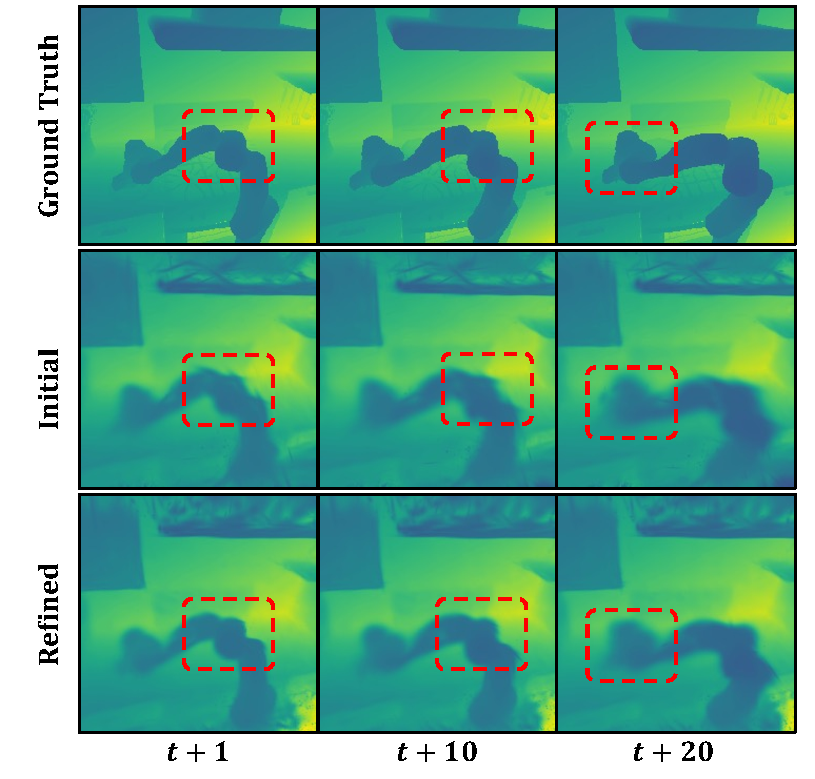
\includegraphics[width=0.47\textwidth]{fig/vis.pdf}
  \vspace{-5pt}
  \caption{\textbf{Qualitative Comparisons of Future Depth Rendering.} Visualizations are shown for timesteps $t+1, t+10, \text{and } t+20$. \textcolor{red}{Red boxes} highlight the improvements in fine-grained geometric details. Best viewed zoomed in.}
  \vspace{-10pt}
  \label{fig:vis}
\end{figure}



\begin{table}[t]
\centering
\small
\caption{\textbf{Real-World Experiment Results.} Task success rates (\%) across three distinct settings: Spatial, Geometry, and Robustness.}
\vspace{-5pt}
\begin{tabular}{l | c c c}
\toprule
\textbf{Method} & \textbf{Spatial} & \textbf{Geometry} & \textbf{Robustness}\\
\midrule
$\pi_0$ (Baseline)~\cite{black2410pi0} & 60.0 & 50.0 & 35.0  \\
\textbf{GeoPredict (Ours)} & 85.0 & 95.0 & 90.0 \\
\bottomrule
\end{tabular}
\label{tab:real}
\vspace{-7pt}
\end{table}


\subsection{Real-World Experiments} \label{sec:real_world}
We validate GeoPredict on a DISCOVER robotic arm to assess performance on tasks demanding explicit 3D reasoning. As detailed in Table~\ref{tab:real}, GeoPredict significantly outperforms the $\pi_0$~\cite{black2410pi0} baseline across all tasks. Specifically, in the Spatial and Robustness tasks, our method achieves success rates of 85.0\% and 90.0\% respectively, surpassing the baseline scores of 60.0\% and 35.0\% and demonstrating superior spatial generalization and resilience to distractors. In the Geometry task, GeoPredict attains a 95.0\% success rate compared to 50.0\% for the baseline. This 45.0\% improvement on tasks involving object sizes absent from the training set strongly indicates that our predictive 3DGS module endows the policy with a generalizable understanding of 3D geometry, enabling adaptive grasping capabilities that the 2D-centric $\pi_0$ baseline lacks. Moreover, since our method explicitly encodes motion history via the Track Encoder, the Appendix provides a dedicated real-world experiment to validate the effectiveness of this historical context.
